\chapter{Implementaciones}

\begin{comment}
Aca describo el kernel y aspectos relevantes de las versiones implementadas:
-que variables tengo que tener en cuenta en las implementaciones(por ej. el tamaño de la tabla,el rango, etc)
-que resultados espero!
-como afecta la periodicidad. la describo aca o en la parte de resultados??
-como afecta el tamaño de los bloques
\end{comment}

En este capítulo se describen los aspectos relevantes de las implementaciones realizadas, correspondientes al algoritmo detallado en las secciones previas, incluyendo también las variantes planteadas y
detallando cómo se tuvieron en cuenta los aspectos de performance propios de la arquitectura GPU, expuestos en el capítulo 2.

Si bien las modificaciones están centradas puntualmente en la etapa de cálculo de las fuerzas, y la evaluación de la performance se realizará sobre este paso,
se describen aspectos de implementación de todo el método ya que son relevantes para evaluar, luego, la correctitud numérica de los resultados.
% , la cual depende de todos los pasos en la iteración global.

% Se describen, entonces, aspectos de la implementación correspondientes a las modificaciones que este trabajo plantea, junto con algunas optimizaciones propias de la implementación base sobre GPU, 
% que no serán evaluadas pero igualmente formaron parte de la implementación final y de la investigación realizada para este trabajo.


\section{Consideraciones previas}

\subsubsection{Precisión numérica}

Una de las primeras decisiones que se deben considerar es la precisión que se utilizará para realizar los cálculos de interacciones individuales y para acumular los resultados de fuerzas que actúan sobre una partícula. 
Dadas las caracterísiticas de la arquitectura GPU, esta decisión podrá afectar severamente la eficiencia para realizar el cálculo y, por lo tanto, es uno de los factores mas importantes a analizar.

Estas propiedades ya han sido estudiadas usando distintas implementaciones del métodom, en particular se ha estudiado usando Amber\cite{le2013spfp}. 
El trabajo mencionado analiza un esquema mixto que implica almacenar los cálculos de fuerzas entre particulas utilizando precisión simple, y acumular en variables de precisión doble
la suma de todos los aportes que componen la fuerza sobre una partícula. Asumiendo los resultados en performance y correctitud encontrados y,
dado que es el software con el cual evaluaremos luego la calidad numérica lograda, utilizaremos un esquema similar de precisión para nuestra implementación.
Más adelante en este capítulo veremos que el esquema utilizado es, además, adecuado para almacenar los valores tabulados en el sistema de memoria de la arquitectura.

\subsubsection{Esquema de accesos a memoria}

Las arquitecturas de placas de v\'ideo est\'an dise\~nadas en torno al poder de c\'omputo.
Las decisiones tomadas por los dise\~nadores de las GPUs se concentran alrededor de paralelismo a lo ancho, poniendo un gran \'enfasis en la cantidad de n\'ucleos.
En consecuencia, se dispone de menor cantidad de espacio f\'isico para m\'as memoria.

Esta decisi\'on implica que la amplia mayor\'ia de la memoria de la GPU se encuentra localizada afuera del chip.
Por lo tanto, esconder la gran latencia que tiene al acceder a la misma es parte importante del paradigma de programaci\'on para GPGPUs.

Es cr\'itico, adem\'as, que los accesos a memoria sean a direcciones m\'ultiplos de $16$, esto se conoce como \textit{accesos alineados}.
El t\'ermino \emph{coalescencia de memoria} se define en GPU como la organizaci\'on de los accesos a memoria de manera secuencial, ordenada y predecible.
Cuando la GPU accede a memoria de manera alineada, puede traer $16$, $32$ o $64$ elementos de 32 bits en una sola lectura~\cite{cudaProgrammingGuide}, suficiente para cada uno de los \threads{} del warp.
Si, en cambio, no se respeta la alineaci\'on de la memoria o los \threads{} tienen un patr\'on de pedidos impredecible, entonces se deber\'an serializar los accesos y separar en m\'ultiples transacciones a memoria global para satisfacerlos.
Este problema se agrava si se deben hacer accesos frecuentes por cientos de \threads{}, como es el caso de los bloques con gran nivel de paralelismo expl\'icito.

Estas propiedades son sumamente importantes para la implementación del algoritmo de dinámica molecular dado que, como se vió hasta ahora, la simplicidad de los cálculos individuales, el gran nivel de paralelismo explícito y 
la cantidad de procesadores disponibles hacen que sea posible computar los resultados en forma muy eficiente para una gran cantidad de partículas, pero, al mismo tiempo, esto genera un cuello de botella al tener que leer y 
escribir una enorme cantidad de datos en memoria. La organización de los accesos a memoria será una parte central en la implementación del algoritmo y del análisis de los resultados que se muestran en el próximo capítulo.

\subsubsection{Propiedades avanzadas de la cache de textura} \label{texturaDetallado}

El centro de las modificaciones planteadas está en el uso de valores tabulados, por lo tanto, independientemente del tamaño y las propiedades de la tabla, teniendo en cuenta que se accederá una gran cantidad de veces a estos datos, 
es importante que el acceso a los datos sea ejecutado de manera sumamente eficiente.
Para implementar este mecanismo hay varias propiedades del sistema de memoria que se puede usar y que se deben analizar, principalmente asociadas a la cache de textura. 

Además del incremento en la eficiencia que provee tener un esquema de memoria cache, la localidad y el concepto de dimensiones que introduce la textura la hacen óptima para accesos a estructuras de datos, 
en particular organizados en 2 dimensiones. En el capítulo 1 (sección \ref{esquemaMemoria}) se mencionó, además, que los accesos a memoria global a través de la cache de textura se resuelven mediante una unidad propia de resoluci\'on de direcciones. 
Esto también será relevante en nuestra implementación, ya que evita tener que realizar cálculos extra para resolver los accesos a la tabla.

Por otro lado, hay algunas propiedades que no se mencionaron previamente pero que son de gran importancia para este trabajo(y para cualquier implementación que requiera del uso de valores tabulados). 
Las mas relevantes son los diferentes modos de direccionamiento que permite la textura en el acceso a los datos, y los filtros que se pueden aplicar sobre éstos al leerlos. 

Los modos de direccionamiento permiten definir como se manejan los accesos a memoria que caen fuera del rango de entradas de la tabla.
En nuestro algoritmo, las tablas contendrán siempre valores resultantes de ecuaciones continuas, por lo que el esquema más natural será asignar el mayor o el menor valor de la tabla cuando se exceda el limite superior o no se alcance el limite inferior, respectivamente. 
Este modo de direccionamiento se conoce como \textit{clamp}
% Además de este modo de direccionamiento, conocido como clamp, existen otras formas de 
% DIRECCIONAMIENTO *****************
% The addressing mode. It is valid to call the device functions of Section B.8 with coordinates that are out of range. 
% The addressing mode defines what happens in that case. The default addressing mode is to clamp the coordinates to the valid range: [0, N) for non-normalized coordinates and [0.0, 1.0) for normalized coordinates.
% NOSOTROS USAMOS ESTE MODO CLAMP
% If the border mode is specified instead, texture fetches with out-of-range texture coordinates return zero. For normalized coordinates, the warp mode and the mirror mode are also available. 
% When using the wrap mode, each coordinate x is converted to frac(x)=x floor(x) where floor(x) is the largest integer not greater than x. 
% When using the mirror mode, each coordinate x is converted to frac(x) if floor(x) is even and 1-frac(x) if floor(x) is odd. 
% The addressing mode is specified as an array of size three whose first, second, and third elements specify the addressing mode for the first, second, and third texture coordinates, respectively; 
% the addressing mode are cudaAddressModeBorder, cudaAddressModeClamp, cudaAddressModeWrap, and cudaAddressModeMirror; cudaAddressModeWrap and cudaAddressModeMirror are only supported for normalized texture coordinates

  
  
% FILTROS ******************************
% The filtering mode which specifies how the value returned when fetching the texture is computed based on the input texture coordinates.
% Linear texture filtering may be done only for textures that are configured to return floating-point data. It performs low-precision interpolation between neighboring texels. 
% When enabled, the texels surrounding a texture fetch location are read and the return value of the texture fetch is interpolated based on where the texture coordinates fell between the texels.
En cuanto a los distintos filtros que se pueden aplicar, los más usuales son el modo puntual, que devuelve el valor con el indice más cercano, y el modo lineal, 
que realiza una interpolación lineal entre el valor superior e inferior en el arreglo(en el caso de 1D). 
Este último filtro es el que aplicaremos para nuestra aproximación, ya que provee una mayor precisión en los resultados para la función con la que estamos trabajando.



% otra ventaja de la memoria de textura es que:
% If the memory reads do not follow the access patterns that global or constant memory reads must follow to get good performance, higher bandwidth can be achieved providing that there is locality in the texture fetches or surface reads;




\section{Implementación base sobre GPU}
El esquema general utilizado para implementar el algoritmo sobre GPU es el explicado en \cite{friedrichs2009accelerating}. 
Sin embargo, en el trabajo mencionado, el potencial incluye componentes de interacción de unión entre partículas, por lo que los cálculos requeridos son algo distintos.
En el capítulo previo se explicaron en detalle los pasos del algoritmo y las ecuaciones a resolver. En esta sección nos centraremos en las variantes de implementación que utilizamos para cada paso.

Para el cálculo de distancias entre partículas, la implementación es bastante directa. La granularidad usada es de un thread por cada par interacción(cada par de partículas) y se usaron tamaños de bloques fijos de $1024\times1$ 
(este tamaño de bloques se mantiene para todos los kernels del algoritmo).
% [1024,1].
% Usando este esquema, con cualquier placa actual es posible lanzar en paralelo el calculo de todas las distancias para sistemas de hasta Xxx partículas. 
Teniendo en cuenta que el cálculo a realizar es  simple y no presenta posibilidades de divergencia, es importante centrar la atención en el esquema de acceso a memoria para logar un uso óptimo de los recursos.

El paso correspondiente al cálculo de las fuerzas entre partículas es, quizás, el más complicado de implementar. El número de implementaciones existentes en la literatura es muy diversa, 
principalmente debido a que los cálculos a realizar dependen del modelo de interacción subyacente, dando lugar a una gran variedad de posibles optimizaciones \cite{friedrichs2009accelerating}\cite{gotz2012routine}\cite{salomon2013routine}.

En el caso de interacciones \textit{non-bond}, como las que se analizan en nuestro trabajo, la principal optimización deriva de la propiedad de simetría que presenta el potencial de interacción.
Es decir, la interacción entre un par de partículas $a$ y $b$ tiene el mismo módulo pero signo opuesto que el valor de ésta entre $b$ y $a$. 
Esto tiene una implicación relevante en el número de cálculos que deben realizarse ya que sólo deberán calcularse interacciones para la mitad de las combinaciones entre partículas, reduciendo así considerablemente el número de cálculos.

Haciendo uso de la propiedad de simetría, entonces, el cálculo de la fuerza resultante de la interacción sólo se realiza $\frac{N^2}{2}$ veces, y el resto se deriva negando este valor.

% Para descomponer las componentes el cálculo se realiza usando un thread por cada par de partículas.

La suma de la fuerza resultante se realiza mediante un esquema de reducción \cite{cudaReductions}. Los threads ponen el resultado de cada interacción individual en su posición correspondiente de la memoria compartida,
evitando tener que realizar operaciones de sincronización entre ellos. Los valores parciales se reducen, luego, con un algoritmo paralelo en árbol: cada thread suma el valor de la posición x con el valor en 2x si este existiera. Esto se repite por la mitad de los threads, hasta que todos los valores hayan sido sumados 
y el thread 0 del bloque escribe el resultado a la memoria global.
Un esquema simplificado de esto puede verse en la figura \ref{reduction}
\begin{figure}[htbp]
   \centering
   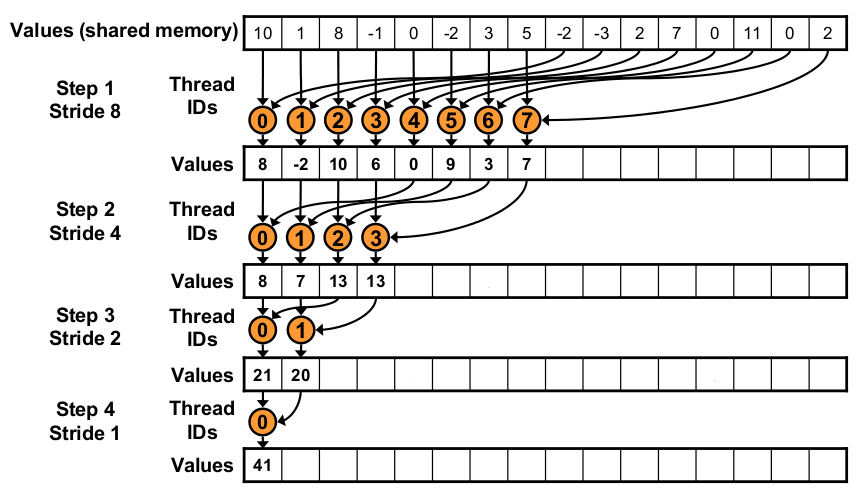
\includegraphics[width=\plotwidth]{img/md/reductions.png}
   \caption{}
   \label{reduction}
\end{figure}

Esta técnica de reducción es sumamente conocida para arquitecturas distribuidas, generando la respuesta en $O(\log_2{n})$ pasos.

Los pasos siguientes son bastante directos ya que requieren, principalmente, actualizaciones de valores en memoria (velocidades, coordenadas). 
Es necesario asegurar un esquema de acceso a memoria apropiado para la gran cantidad de datos que se leen/escriben en sistemas con un número considerable de partículas.  
% La aceleración se calcula en base a la fuerza resultante usando un thread por cada partícula.
% La actualización de coordenadas también se realiza usando un thread para cada partícula. El esquema de threads utilizado asegura acceso coalescente a las matrices de datos asociadas al sistema.

% Para el caso de condiciones periódicas, sin embargo, hay un paso extra que se debe considerar

\section{Implementación usando tabla de potenciales}
% \subsubsection{Tabla sobre memoria global}
% \subsubsection{Tabla sobre memoria de textura}

% 
% Se implementaron variantes equivalentes para el calculo usando la ecuación derivada, usando una tabla de valores potenciales, y usando una tabla de valores de derivada.
% Deberán tenerse en cuenta a la hora de usar esta implementación todos los aspectos asociados a la transferencia de datos entre la memoria del dispositivo y la memoria del host. En el próximo capitulo se verá como esta implementación es utilizada para demostrar las ventajas q aporta la arquitectura GPU.

% claramente los accesos a eta memoria no seguiran un patron que provea coalescencia en el acceso a memoria (el indice de los accesos a memoria estara dado por la distancia y estas tienen una distribucion que no conocemos)
% tener la tabla en memoria provocaria un gran cuello de botella cuando todos los threads intenten a acceder a posiciones de memoria distribuidas en todo el arrreglo

% ****ACA PONGO LAS CARACTERISTICAS QUE OFRECE LA GPU Y QUE PUEDEN SER USADAS APROVECHANDO QUE HOY EN DIA LA MAYORIA DEL SOFT. ESTA IMPLEMENTADO SOBRE GPU*****

Dado que esta modificación plantea reemplazar cálculos por la obtención de los resultados directamente desde memoria, 
para entender su implementación se debe hacer foco en la organización de la memoria en la GPU, en particular en las propiedades de la cache de textura detalladas en la sección \ref{texturaDetallado}.



% ACLARAR QUE SE UTILIZA UN ARREGLO DE 2D, PARA APROVECHAR EL MAYOR TAMAÑO QUE PERMITE UN ARREGLO DE 2 DIMENSIONES:
% para 2D el maximo es: 65536 x 65535
% para 3D el maximo es: 4096 x 4096 x 4096    ( para capabilities 2.x es  2048 x 2048 x 2048 ) 
% DE ESTA FORMA EL FETCH SE HACE EN MODO DE INTERPOLACION SOBE 2D 
% EXPLICAR QUE DADO EL NUMERO DE VARIANTES EN LAS COMBINACIONES DE TIPOS DEL SISTEMA DE PARTICULAS, ES PREFERIBLE TENER 2D BLA BLA BLA....................


La tabla de potenciales se alojará en una estructura de 2 dimensiones asociada a la cache de textura. 
Si bien los valores del potencial varían, como se mencionó en el capítulo previo, en función de tres variables, hay algunas consideraciones adicionales que llevan a tomar esta decisión:

\begin{itemize}
\item La arquitectura impone un limite en el tamaño de los arreglos asociados a la memoria de textura. 
Este límite, tal como se define en las especificaciones técnicas \cite{cudaProgrammingGuide}, es de $65536 \times 65535$ elementos en punto floatante para arreglos de 2 dimensiones, 
y de $4096 \times 4096 \times 4096$ elementos de punto flotante para arreglos de 3 dimensiones (en capabilities 2.x este valor se reduce a $2048 \times 2048 \times 2048$)


\item El objetivo es maximizar el número de valores de $r$ en la tabla, lo que dará una mayor precisión al resultado, al mismo tiempo se deben almacenar todas las combinaciones de pares $\sigma$-$\epsilon$.

\item El número combinaciones de $\sigma$-$\epsilon$ depende de la variabilidad en los tipos de partículas que se están simulando y este valor está en el orden de las decenas.

\end{itemize}

Teniendo esto en cuenta


% El kernel que permite calcular los valores de derivada del potencial utilizando esta tabla se encuentra detallado en la figura \ref{code:potentialsKernel}

Se han dado hasta aquí suficientes detalles acerca de los aspectos relevantes asociados a la implementación sobre GPU, por lo tanto, para evitar una descripción textual que podría extenderse demasiado, se incluye en el cuadro de código \ref{code:potentialsKernel}, 
la implementación correspondiente al kernel que realiza la evaluación de las derivadas a partir de los valores tabulados.

\begin{figure}[htbp]
    \begin{lstlisting}
__global__ void potentialsMode_texture_kernel(
  float* dEr,
  float* r, 
  float cut, 
  int* item_to_type, 
  int num_samples_r, 
  int num_types, 
  int width, 
  int height)
  {
    /* Elemento de la matriz a calcular */
    /** particula 2 **/
    unsigned int x = blockIdx.x * blockDim.x + threadIdx.x;	
    /** particula 1 **/
    unsigned int y = blockIdx.y * blockDim.y + threadIdx.y;
    
    float rvalue= r[y*width+x]; 
    float result;
    
    /* Asegurarse que el thread esta dentro de los valores a calcular */
    if(x >= width || y >= height) {return;}
    if(x == y || rvalue  >= cut) 
      {
	result=0;  //fuera del cutoff
      }
      else{
      //indice 1 matriz de tipos de interacciones
      float t_o_p_1 = (float) item_to_type[y] * num_types;	
      
      //indice 2 de la matriz de tipos de interacciones
      float t_o_p_2 =  item_to_type[x] + 0.5 + t_o_p_1;	
      
      // convertir r en indice
      float index_x = ((rvalue - MIn) * (num_samples_r / DIST + 0.5);	
      
      //fetch valores de potencial
      float E_r_up = tex2D( texRef, index_x + DIF_FINITAS_DELTA, t_o_p_2 );
      float E_r_dwn = tex2D( texRef, index_x - DIF_FINITAS_DELTA, t_o_p_2 );
      float r_dif = DIST * 2 * (DIF_FINITAS_DELTA) / num_samples_r;
      
      //DERIVADA DISCRETIZADA
      result = (E_r_up - E_r_dwn) / (r_dif); 
      }
   
    //ESCRIBIR RESULTADOS
    dEr[y*width+x]= result;
}
    \end{lstlisting}
    \caption{Kernel utilizado para el cálculo de fuerzas a partir de una tabla de potenciales en textura}
    \label{code:potentialsKernel}
\end{figure}

La mayor parte de éste se puede entender directamente ya que está en el lenguaje C base. Además de esto, en las líneas ...
% PONER LAS LINEAS QUE TIENEN ALGUNA FUNCION CUDA PUNTUAL


\section{Implementación usando tabla de derivadas}
% \subsubsection{Tabla sobre memoria global}
% \subsubsection{Tabla sobre memoria de textura}


El kernel que permite calcular los valores de derivada del potencial utilizando esta tabla se encuentra detallado en la figura \ref{code:derivativesKernel}

\begin{figure}[htbp]
    \begin{lstlisting}
__global__ void direct_derivativeMode_E_r (
    float* dEr,
    float* r, 
    float cut, 
    int* item_to_type, 
    int num_samples_r, 
    int num_types, 
    int width, 
    int height )
{ 
  /* Elemento de la matriz a calcular */
   /** particula 2 **/
  unsigned int x = blockIdx.x * blockDim.x + threadIdx.x;
  
  /** particula 1 **/
  unsigned int y = blockIdx.y * blockDim.y + threadIdx.y;	
  float rvalue= r[y*width+x]; 
  float result;
  
  /* Asegurarse que el thread esta dentro de los valores a calcular */
  if(x >= width || y >= height) {return;}
  if(x == y || rvalue  >= cut) 
    {
      result=0;  //fuera del cutoff
    }
    else{
      //indice 1 matriz de tipos de interacciones
      float t_o_p_1 =  item_to_type[y] * num_types;	
      
      //indice 2 matriz de tipos de interacciones
      float t_o_p_2 =  item_to_type[x] + 0.5 + t_o_p_1;	
      
      // convertir r en indice
      float index_x = ( (rvalue - MIn) * num_samples_r / DIST + 0.5);	
     
      //fetch result
      result = tex2D( texRef, index_x, t_o_p_2 );
    }
   
  //ESCRIBIR RESULTADO 
  dEr[y*width+x]= result;

}
    \end{lstlisting}
    \caption{Kernel utilizado para el cálculo de fuerzas a partir de una tabla de derivadas en textura}
    \label{code:derivativesKernel}
\end{figure}



\section{Implementacion sobre CPU}

Con el fin de poder hacer una comparación real de los aspectos asociados a la performance se desarrolló además una implementación que realiza el cálculo de fuerzas sobre CPU.

Esta implementación solo modifica la forma en que se calcula la derivada del potencial, la cual se ejecuta ahora sobre la CPU, por lo tanto los datos de distancia y potenciales deben estar accesibles en memoria para que este cálculo pueda ser realizado.
